\documentclass[11pt]{article}

\usepackage[T1]{fontenc}
\usepackage[margin=1in]{geometry}
\usepackage{amsmath,amssymb,amsthm,mathtools}
\IfFileExists{newtxtext.sty}{%
  \usepackage{newtxtext,newtxmath}%
}{%
  % Portable fallback for minimal TeX Live installations.
  \usepackage{mathptmx}%
}
\usepackage{microtype}
\usepackage{booktabs}
\usepackage{enumitem}
\usepackage{placeins}
\usepackage{tikz}
\usetikzlibrary{arrows.meta,calc,positioning}
\usepackage{xcolor}
\usepackage[
  colorlinks=true,
  linkcolor=blue!45!black,
  citecolor=blue!45!black,
  urlcolor=blue!45!black
]{hyperref}

\allowdisplaybreaks
\setlist[itemize]{leftmargin=1.6em,itemsep=0.2em,topsep=0.4em}
\setlist[enumerate]{leftmargin=1.8em,itemsep=0.2em,topsep=0.4em}

\newtheorem{theorem}{Theorem}[section]
\newtheorem{proposition}[theorem]{Proposition}
\newtheorem{lemma}[theorem]{Lemma}
\newtheorem{corollary}[theorem]{Corollary}
\theoremstyle{definition}
\newtheorem{definition}[theorem]{Definition}
\theoremstyle{remark}
\newtheorem{remark}[theorem]{Remark}

\newcommand{\R}{\mathbb{R}}
\newcommand{\cert}{\mathcal{H}}
\newcommand{\smoothclass}{\mathcal{F}}
\newcommand{\invprod}{\Pi}
\newcommand{\rankmass}{M}
\newcommand{\rankdens}{d}
\newcommand{\rankgain}{g}
\newcommand{\criticalexp}{\beta_{\star}}
\newcommand{\gdexp}{\beta_{\mathrm{GD}}}
\newcommand{\threshold}{d_{\star}}
\newcommand{\rankcut}{q_{\star}}
\newcommand{\ent}{\operatorname{ent}}
\newcommand{\argmin}{\operatorname*{argmin}}
\newcommand{\dist}{\operatorname{dist}}
\newcommand{\lbconst}{c_{\mathrm{lb}}}
\newcommand{\propconst}{\Gamma_{\mathrm{prop}}}

\title{\bfseries
A Lower Bound at Exponent \(\sqrt{3}\) for Predetermined-Stepsize Gradient Descent}
\author{Zuang Wang and Dandan Wang}

\begin{document}
\maketitle

\begin{abstract}
We study the last iterate of gradient descent on convex \(L\)-smooth
functions when the entire nonnegative stepsize schedule is fixed before any
oracle information is observed.  Our proof uses a marked-stage realization
and rank-cutoff framework that also appears in Ma and Chen, who give universal
lower bounds with every exponent \(\gamma>\sqrt{2+\sqrt3}\)
\cite{machen2026}.  Relative to their argument, our new ingredient is a
direct entropy bound for the full,
unrelaxed temporally ordered reciprocal product; it replaces their
budget-equalization and two-matching bound.  We prove that there is an
absolute constant
\(\lbconst>0\)
such that, for every horizon \(T\), every predetermined nonnegative schedule,
and every prescribed initialization, one can construct an instance in
dimension at most \(T+1\) satisfying
\[
 f(x_T)-f^\star
 \ge \lbconst LR^2(T+1)^{-\sqrt3}.
\]
The lower-bound proof is self-contained: the citations to Ma and Chen record
provenance, while every shared component used below is rederived in full and
no result from their paper is invoked as a premise.

Starting from exact local and terminal identities proved below, and also
present in Ma--Chen, the proof retains the full temporal inverse product
associated with the selected long steps.  A two-state
entropy inequality telescopes along the full selected path, cancels all
interior entropy terms, and reduces the product estimate to a uniformly
controlled pair of endpoint states.  This yields a critical-density
alternative at density \(1/2\); cutoff propagation and a finite-cutoff
argument then close at exponent \(\sqrt3\).  The gap to the silver-schedule
upper exponent \(\log_2(1+\sqrt2)\) remains open. We use ChatGPT 5.6 Pro and
ChatGPT 5.6 Sol Ultra for developing part of the proof for this paper.
\end{abstract}

\section{Introduction}
\label{sec:introduction}

We consider unconstrained minimization of a convex function
\(f:\R^d\to\R\) whose gradient is \(L\)-Lipschitz.  Gradient descent (GD)
takes the form
\begin{equation}
 x_{t+1}=x_t-\eta_t\nabla f(x_t),
 \qquad 0\le t<T.
 \label{eq:physical-gd}
\end{equation}
A schedule is \emph{predetermined} when the complete vector
\((\eta_0,\ldots,\eta_{T-1})\in\R_{\ge0}^T\) is fixed before any function
value or gradient is observed.  It may depend on the announced horizon and
on \(L\), and it may be nonmonotone and contain arbitrarily large steps, but
it cannot react to the realized oracle transcript.

Classical stable steps give an \(O(T^{-1})\) last-iterate guarantee for
smooth convex minimization.  Carefully arranged long steps can do better.
Although an individual long step may increase the objective, interactions
among many such steps can yield a faster global rate.  In particular, silver
schedules attain the exponent \(\log_2(1+\sqrt2)\), and concatenation
constructions extend that guarantee to arbitrary announced horizons
\cite{altschuler2025silver,zhangjiang2024}.  This raises a restricted
minimax question: how fast can plain GD converge when only its scalar
stepsizes may be designed in advance?

A lower bound with exponent \(\beta_{\rm lb}\) means that every schedule
has an instance whose error is at least a constant multiple of
\(T^{-\beta_{\rm lb}}\).  A smaller lower-bound exponent is therefore
stronger: it rules out every uniform upper rate
\(O(T^{-\beta_{\rm up}})\) with
\(\beta_{\rm up}>\beta_{\rm lb}\).  This reverses the visual ordering
familiar from upper bounds and makes a precise minimax definition useful.

\subsection{Minimax formulation and main result}

We first remove the inessential scale parameters.  For \(d\ge1\), a
prescribed point \(z\in\R^d\), and a dimensionless schedule
\(\alpha=(\alpha_0,\ldots,\alpha_{T-1})\in\R_{\ge0}^T\), let
\(x_t^{f,\alpha,z}\) denote the
iterates
\[
 x_0^{f,\alpha,z}=z,\qquad
 x_{t+1}^{f,\alpha,z}
 =x_t^{f,\alpha,z}-\alpha_t\nabla f(x_t^{f,\alpha,z}).
\]
Let \(\smoothclass_1(\R^d)\) be the class of convex functions on \(\R^d\)
with
\(1\)-Lipschitz gradient, and define the worst-case normalized last-iterate
error
\begin{equation}
 \mathcal R_{T,d}(\alpha;z)
 :=
 \sup_{\substack{
       f\in\smoothclass_1(\R^d),\ x_\star\in\argmin f\\
       \|z-x_\star\|=1}}
 \bigl\{f(x_T^{f,\alpha,z})-f(x_\star)\bigr\}.
 \label{eq:fixed-initialization-risk}
\end{equation}
This value is independent of \(z\).  Indeed, for \(z,z'\in\R^d\), the
translation
\[
 f'(x):=f(x+z-z'),
 \qquad
 x_\star':=x_\star-z+z'
\]
is a bijection between the instances in
\eqref{eq:fixed-initialization-risk} at \(z\) and at \(z'\), and it
translates the entire GD trajectory without changing any function-value
gap.  We may therefore fix the prescribed initialization to be the origin
\(0_d\) in each dimension.

The horizon-\(T\) minimax value is
\begin{equation}
 \mathcal M_T
 :=
 \inf_{\alpha\in\R_{\ge0}^T}
 \max_{1\le d\le T+1}
 \mathcal R_{T,d}(\alpha;0_d).
 \label{eq:minimax-value}
\end{equation}
Thus the schedule is chosen before the adversarial instance and dimension,
while the hard instance may depend on the schedule.  The normalization loses
no generality: for physical parameters \(L,R>0\), set
\(\alpha_t=L\eta_t\) and
apply the translation and scaling in Section~\ref{sec:scaling}.

\begin{definition}[Horizon-dependent minimax exponent]
\label{def:minimax-exponent}
The minimax exponent is
\begin{equation}
 \gdexp
 :=
 \sup\left\{
 \beta\ge0:
 \begin{array}{l}
 \text{there is a constant \(C_\beta<\infty\), independent of \(T\), such that}\\[-1mm]
 \mathcal M_T\le C_\beta(T+1)^{-\beta}\quad\text{for every \(T\ge1\)}
 \end{array}
 \right\}.
 \label{eq:minimax-exponent}
\end{equation}
\end{definition}
The defining set is nonempty: the zero schedule and the smoothness
inequality give \(\mathcal M_T\le1/2\).  The infimum in
\eqref{eq:minimax-value} is taken separately at each announced horizon.
Thus \(\gdexp\) describes horizon-dependent schedules; an
anytime exponent, which would require one infinite schedule whose prefixes
work simultaneously at every horizon, is a different quantity.

\begin{theorem}[Universal \(\sqrt3\) lower bound]
\label{thm:main}
There is an absolute constant \(\lbconst>0\) such that the following holds.
For every \(T\ge1\), every \(L,R>0\), and every predetermined schedule
\((\eta_t)_{t=0}^{T-1}\in\R_{\ge0}^T\), there is a dimension
\(d\le T+1\) such that, for every prescribed
\(x_{\rm init}\in\R^d\), there exist a convex \(L\)-smooth function
\(f:\R^d\to\R\) and a point \(x_\star\in\argmin f\) satisfying
\(\|x_{\rm init}-x_\star\|=R\) for which GD initialized at
\(x_0=x_{\rm init}\) obeys
\begin{equation}
 f(x_T)-f(x_\star)
 \ge \lbconst LR^2(T+1)^{-\sqrt3}.
 \label{eq:main-bound}
\end{equation}
The function and minimizer may depend on the prescribed schedule and
initialization, but the constant \(\lbconst\) does not.
\end{theorem}

\begin{corollary}[Minimax consequence]
\label{cor:minimax-consequence}
For every \(T\ge1\),
\[
 \mathcal M_T\ge\lbconst(T+1)^{-\sqrt3},
 \qquad
 \gdexp\le\sqrt3.
\]
Together with the arbitrary-horizon silver-schedule upper bound
\cite{altschuler2025silver,zhangjiang2024}, this gives
\begin{equation}
\boxed{
 \log_2(1+\sqrt2)
 \le \gdexp
 \le \sqrt3.}
 \label{eq:minimax-exponent-bracket}
\end{equation}
\end{corollary}

\begin{proof}
Apply Theorem~\ref{thm:main} with \(L=R=1\) to each
\(\alpha\in\R_{\ge0}^T\), take the maximum over \(1\le d\le T+1\), and then
take the infimum over \(\alpha\).  This proves the lower bound on
\(\mathcal M_T\).

If some \(\beta>\sqrt3\) belonged to the set in
Definition~\ref{def:minimax-exponent}, then for a constant \(C_\beta\)
independent of \(T\),
\[
 \lbconst(T+1)^{-\sqrt3}
 \le\mathcal M_T
 \le C_\beta(T+1)^{-\beta}
\]
for every \(T\), which is impossible as \(T\to\infty\).  Hence
\(\gdexp\le\sqrt3\).  The cited arbitrary-horizon
silver-schedule guarantee places \(\log_2(1+\sqrt2)\) in the closure of
the achievable upper exponents and proves the opposite inequality.  This
left-hand inequality is the only externally supplied implication in the
corollary; it is not used for Theorem~\ref{thm:main} or for
\(\gdexp\le\sqrt3\).
\end{proof}

The exponent comparison is summarized in Table~\ref{tab:exponents}.  For
the lower-bound rows, the smaller exponent gives the stronger restriction.

\begin{table}[ht]
\centering
\begin{tabular}{@{}lll@{}}
\toprule
Result & exponent & numerical value\\
\midrule
Silver-schedule upper bound
  \cite{altschuler2025silver,zhangjiang2024}
  & \(s=\log_2(1+\sqrt2)\) & \(1.2715533\ldots\)\\
Theorem~\ref{thm:main}
  & \(\criticalexp=\sqrt3\) & \(1.7320508\ldots\)\\
Ma--Chen (2026) lower bound \cite{machen2026}
  & every \(\gamma>\sqrt{2+\sqrt3}\) & \(\gamma>1.9318517\ldots\)\\
\bottomrule
\end{tabular}
\caption{Upper and lower exponents for horizon-dependent last-iterate
convergence.}
\label{tab:exponents}
\end{table}

\subsection{Related work}

\paragraph{Stepsize-only acceleration.}
Predetermined, time-varying stepsizes can accelerate plain GD even when
occasional steps are large enough that a single iteration need not decrease
the objective
\cite{grimmer2024long,altschulerparrilo2025hedging,
altschuler2025silver,grimmershuwang2025long}.
Altschuler and Parrilo introduced the recursive silver schedule in the
strongly convex setting and subsequently proved, for smooth convex
optimization, the last-iterate rate
\(O(T^{-\log_2(1+\sqrt2)})\) at horizons \(T=2^k-1\)
\cite{altschulerparrilo2025hedging,altschuler2025silver}.
Grimmer, Shu, and Wang obtained the same exponent for objective-gap and
squared-gradient-norm guarantees using related long-step schedules
\cite{grimmershuwang2025long}.  Concatenation and composition constructions
extend this exponent to every prescribed horizon
\cite{zhangjiang2024,grimmershuwang2025compose}.

\paragraph{Lower bounds and the oracle model.}
General accelerated first-order methods attain the \(O(T^{-2})\) rate
\cite{nesterov1983}, and the corresponding information-based
\(\Omega(T^{-2})\) lower bound is tight for the full first-order oracle class
in sufficiently high dimension \cite{drori2016}.  That general lower bound
allows algorithms to combine past oracle information and therefore does not
distinguish plain GD from accelerated methods.  Structure-specific lower
bounds for time-invariant oblivious algorithms were given by Arjevani and
Shamir \cite{arjevanishamir2016}; they do not cover arbitrary time-varying
stepsize schedules.  Grimmer, Shu, and Wang prove matching lower bounds
within their restricted class of basic composable schedules
\cite{grimmershuwang2025compose}.

\paragraph{Anytime versus prescribed-horizon schedules.}
An anytime guarantee uses one infinite stepsize sequence, independent of the
stopping time, and must hold at every stopping time.  This differs from
\eqref{eq:minimax-value}, where the length-\(T\) schedule may depend on the
announced horizon.  Kornowski and Shamir posed whether anytime stepsize-only
acceleration is possible \cite{kornowskishamir2024}.  Zhang, Lee, Du, and
Chen constructed an anytime schedule with objective-gap rate
\cite{zhangetal2025anytime}
\[
 O\!\left(T^{-2s/(1+s)}\right)=O(T^{-1.119\ldots}),
 \qquad s=\log_2(1+\sqrt2),
\]
Tsai, Fatkhullin, Zhang, and He subsequently
proved that no single infinite schedule of strictly positive stepsizes can
have worst-case objective-gap rate \(o(T^{-4/3})\)
\cite{tsaietal2026anytime}.  Their quantifiers and strict-positivity
assumption differ from the present horizon-dependent theorem, which permits
nonnegative stepsizes.

\paragraph{Relation to the Ma--Chen framework.}
Ma and Chen prove that arbitrary predetermined nonnegative schedules admit a
worst-case last-iterate lower bound of order \(T^{-\gamma}\) for every
\(\gamma>\sqrt{2+\sqrt3}\) \cite{machen2026}.  Their proof contains
counterparts of our marked-stage realization, residual-rank statistics,
neighboring-cutoff recurrences, Lyapunov transport, and bounded-rank prefix
estimate.  We rederive each below; the citations record provenance, not
logical dependence.  Our distinct component is a direct two-state entropy
bound for the full, unrelaxed ordered reciprocal product.  It replaces their
budget equalization, auxiliary terminal vertex, and matching analysis, yields
the half-density certificate, and closes at \(\sqrt3\).  Separate notation
clarifies the variables' roles, not a different outer architecture.

\paragraph{Logical self-containedness.}
Theorem~\ref{thm:main} and the inequality
\(\gdexp\le\sqrt3\) do not use any theorem, lemma, or calculation from
Ma--Chen as a black box.  Every paper-specific construction, recurrence,
estimate, and case argument is proved in
Sections~\ref{sec:functional}--\ref{sec:scaling}; hence the result does not
depend on the correctness of \cite{machen2026}.  The cited silver-schedule
bound is used only for the opposite comparison
\(\log_2(1+\sqrt2)\le\gdexp\), not for the lower-bound theorem.

\subsection{Technical contribution and proof roadmap}

\paragraph{Main technical idea.}
Split each dimensionless step into a capped part and a nonnegative surplus,
order the positive surpluses, choose a cutoff prefix, and restore it to
temporal order.  Proposition~\ref{prop:realization} realizes this selection
as a stage chain whose final gap is controlled by local transition factors.
From the exact mass partition and terminal identity
\(\Omega_q=2\omega_{\rm end}-1\), we keep the full ordered reciprocal product
unrelaxed and apply a two-state entropy inequality.  Consecutive endpoint
terms cancel, leaving only the two ends of the chain.

\paragraph{Contribution.}
The direct entropy estimate for the full ordered inverse product proves
\[
 \rankdens_q\le\frac12
 \quad\Longrightarrow\quad
 \cert_T(\alpha)\ge\frac1{5\rankmass_q}.
\]
The neighboring-cutoff recurrences and a Lyapunov estimate at
\(\criticalexp=\sqrt3\) propagate this bound through large cutoffs; a
finite-cutoff lemma and complete scan handle the rest.  No optimality is
claimed for the threshold, constant, or exponent.

\paragraph{Proof roadmap.}
Figure~\ref{fig:proof-roadmap} records every numbered result and the two final
transfer steps.  Three scalar branches meet in
Proposition~\ref{prop:schedule-bound}; the geometric branch joins afterward
to realize and rescale the hard instance.

\clearpage
\begin{figure}[t]
\centering
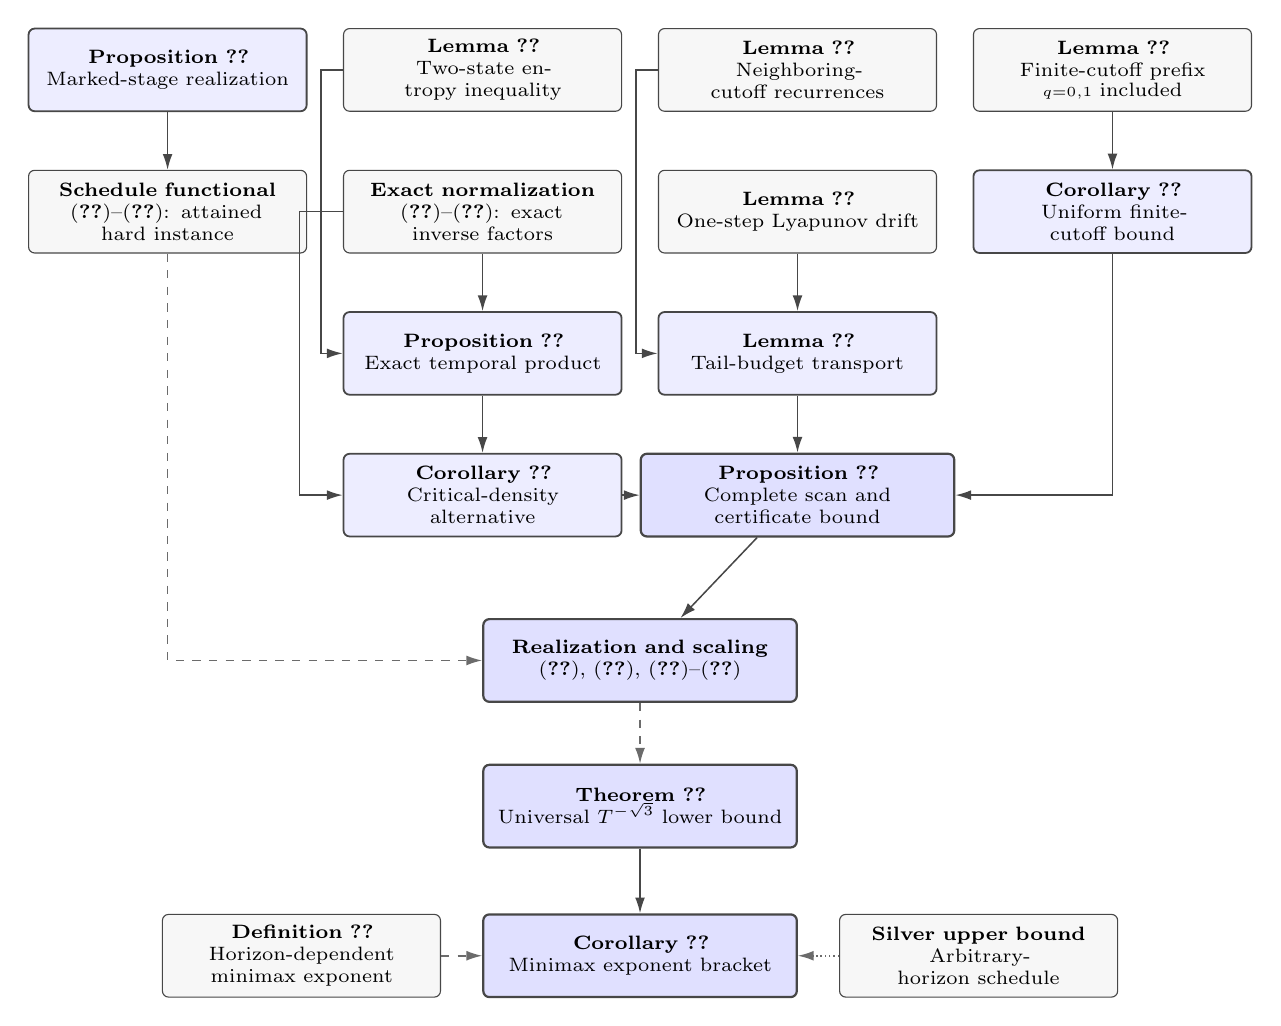
\begin{tikzpicture}[
  result/.style={
    draw=black!72,
    rounded corners=2.2pt,
    align=center,
    inner xsep=4pt,
    inner ysep=3.5pt,
    text width=3.25cm,
    minimum height=1.05cm,
    font=\scriptsize
  },
  ingredient/.style={result,fill=black!3},
  milestone/.style={result,fill=blue!7,line width=0.65pt},
  conclusion/.style={
    result,
    fill=blue!12,
    line width=0.8pt,
    text width=3.7cm
  },
  proof/.style={
    -{Latex[length=2mm,width=1.25mm]},
    draw=black!72,
    line width=0.55pt
  },
  translation/.style={proof,dashed,draw=black!58},
  external/.style={proof,densely dotted,draw=black!58}
]
% Geometric-realization branch
\node[milestone] (realization) at (1.75,0)
  {\textbf{Proposition~\ref{prop:realization}}\\
   Marked-stage realization};
\node[ingredient] (functional) at (1.75,-1.8)
  {\textbf{Schedule functional}\\
   \eqref{eq:C-functional}--\eqref{eq:C-attained}: attained hard instance};

% Exact-product branch
\node[ingredient] (entropy) at (5.75,0)
  {\textbf{Lemma~\ref{lem:entropy-edge}}\\
   Two-state entropy inequality};
\node[ingredient] (normalization) at (5.75,-1.8)
  {\textbf{Exact normalization}\\
   \eqref{eq:mass-partition}--\eqref{eq:C-from-E}: exact inverse factors};
\node[milestone] (product) at (5.75,-3.6)
  {\textbf{Proposition~\ref{prop:global-product}}\\
   Exact temporal product};
\node[milestone] (density) at (5.75,-5.4)
  {\textbf{Corollary~\ref{cor:small-density}}\\
   Critical-density alternative};

% Adjacent-rank branch
\node[ingredient] (recurrences) at (9.75,0)
  {\textbf{Lemma~\ref{lem:rank-recurrences}}\\
   Neighboring-cutoff recurrences};
\node[ingredient] (drift) at (9.75,-1.8)
  {\textbf{Lemma~\ref{lem:drift}}\\
   One-step Lyapunov drift};
\node[milestone] (propagation) at (9.75,-3.6)
  {\textbf{Lemma~\ref{lem:propagation}}\\
   Tail-budget transport};

% Bounded-rank branch
\node[ingredient] (prefix) at (13.75,0)
  {\textbf{Lemma~\ref{lem:bounded-prefix}}\\
   Finite-cutoff prefix\\[-1pt]
   {\(\scriptstyle q=0,1\) included}};
\node[milestone] (bounded) at (13.75,-1.8)
  {\textbf{Corollary~\ref{cor:bounded-rank}}\\
   Uniform finite-cutoff bound};

% Convergence of the schedule branches
\node[conclusion] (scan) at (9.75,-5.4)
  {\textbf{Proposition~\ref{prop:schedule-bound}}\\
   Complete scan and certificate bound};
\node[conclusion] (scaling) at (7.75,-7.5)
  {\textbf{Realization and scaling}\\
   \eqref{eq:B-r-horizon}, \eqref{eq:C-attained},
   \eqref{eq:C-horizon}--\eqref{eq:physical-scaling}};
\node[conclusion] (main) at (7.75,-9.35)
  {\textbf{Theorem~\ref{thm:main}}\\
   Universal \(T^{-\sqrt3}\) lower bound};

% Minimax consequence
\node[ingredient] (definition) at (3.45,-11.25)
  {\textbf{Definition~\ref{def:minimax-exponent}}\\
   Horizon-dependent minimax exponent};
\node[conclusion] (minimax) at (7.75,-11.25)
  {\textbf{Corollary~\ref{cor:minimax-consequence}}\\
   Minimax exponent bracket};
\node[ingredient] (silver) at (12.05,-11.25)
  {\textbf{Silver upper bound}\\
   Arbitrary-horizon schedule};

% Direct proof dependencies
\draw[proof] (realization) -- (functional);
\draw[proof] (entropy.west) -- ++(-0.28,0) |- (product.west);
\draw[proof] (normalization) -- (product);
\draw[proof] (product) -- (density);
\draw[proof] (normalization.west) -- ++(-0.55,0) |- (density.west);
\draw[proof] (drift) -- (propagation);
\draw[proof] (recurrences.west) -- ++(-0.28,0) |- (propagation.west);
\draw[proof] (prefix) -- (bounded);
\draw[proof] (density) -- (scan);
\draw[proof] (propagation) -- (scan);
\draw[proof] (bounded.south) |- (scan.east);
\draw[proof] (scan) -- (scaling);

% Realization/scaling and minimax translations
\draw[translation] (functional.south) |- (scaling.west);
\draw[translation] (scaling) -- (main);
\draw[proof] (main) -- (minimax);
\draw[translation] (definition) -- (minimax);
\draw[external] (silver) -- (minimax);
\end{tikzpicture}
\caption{Proof architecture for Theorem~\ref{thm:main} and
Corollary~\ref{cor:minimax-consequence}.  Solid arrows denote direct internal
proof dependencies; dashed arrows denote realization, definition, or
horizon/scaling transfers; and the dotted arrow denotes the external
silver-schedule input.  The full-product entropy branch is the
product-control replacement introduced here; the realization,
cutoff-dynamics, finite-cutoff, and scan branches have counterparts in
Ma--Chen \cite{machen2026}, but every solid or dashed dependency shown here
is established inside this paper.}
\label{fig:proof-roadmap}
\end{figure}

The realization branch, neighboring-cutoff recurrences, Lyapunov transport,
and finite-cutoff branch have counterparts in the Ma--Chen framework
\cite{machen2026}; their proofs below are complete and use no external
Ma--Chen result.  The full-product entropy branch is the
replacement introduced here: it gives the half-density input to that outer
framework.  On its complement, the neighboring-cutoff recurrences and the
one-step Lyapunov lemma jointly yield tail-budget transport.  The
finite-cutoff branch supplies the remaining finite cases.
Corollary~\ref{cor:small-density},
Lemma~\ref{lem:propagation}, and Corollary~\ref{cor:bounded-rank} are exactly
the three inputs scanned in Proposition~\ref{prop:schedule-bound}.

The edge cases are localized in the diagram as follows.  The empty marked
chain \(J=0\) is included in \eqref{eq:C-functional}; the exact-product
branch is used only for \(q\ge2\); and
Lemma~\ref{lem:bounded-prefix} handles \(q=1\) with an empty internal product
and \(q=0\) through the empty chain.  The \(N<\rankcut\) and small-horizon cases
close through Corollary~\ref{cor:bounded-rank}.  In
Lemma~\ref{lem:propagation}, \(k=N\) is immediate and \(k<N\) uses the core
estimate at \(k_0=k+1\).  Thus the final scan requires neither an undefined
empty product nor a limiting argument from a larger exponent.

\FloatBarrier
\section{The dimensionless certificate functional}
\label{sec:functional}

We first set \(L=R=1\) and write the normalized schedule as
\[
  \alpha_t:=L\eta_t,\qquad 0\le t<T.
\]
The construction below associates a hard convex \(1\)-smooth function with
any numerical vector \(\alpha\in\R_{\ge0}^T\).  The capped-surplus stage
data, realization, and maximized certificate in this section are
notational counterparts of the construction in Sections~4.1--4.4 of Ma and
Chen \cite{machen2026}.  All claims needed from this construction are proved
here, including the exact terminal scale and the empty-chain convention used
later.

\subsection{Step surpluses and stage data}

Separate the capped and excess portions of each step:
\begin{equation}
 \delta_t:=(\alpha_t-1)_+,
 \qquad
 \rankmass_{\mathrm{cap}}
 :=1+\sum_{t=0}^{T-1}\min\{\alpha_t,1\},
 \qquad
 N:=\bigl|\{t:\delta_t>0\}\bigr|.
 \label{eq:base-mass}
\end{equation}
In particular,
\begin{equation}
  \rankmass_{\mathrm{cap}}\le T+1,\qquad N+1\le T+1.
  \label{eq:B-r-horizon}
\end{equation}

Choose \(J\) surplus-bearing indices
\[
 0\le \iota_1<\cdots<\iota_J<T,\qquad \delta_{\iota_j}>0.
\]
When \(J\ge1\), they split the unselected indices into gaps
\[
\begin{aligned}
 \mathcal I_0&=\{0,\ldots,\iota_1-1\},\\
 \mathcal I_i&=\{\iota_i+1,\ldots,\iota_{i+1}-1\},
       &&1\le i<J,\\
 \mathcal I_J&=\{\iota_J+1,\ldots,T-1\}.
\end{aligned}
\]
For \(J=0\), set \(\mathcal I_0=\{0,\ldots,T-1\}\); all nonterminal quantities
below are then absent.
For \(0\le i<J\), define
\begin{equation}
 \omega_i:=1+\sum_{t\in\mathcal I_i}\alpha_t,
 \qquad
 \Omega_i:=\omega_i+\delta_{\iota_{i+1}},
 \label{eq:block-masses}
\end{equation}
and define the terminal scale
\begin{equation}
 \Omega_J:=1+2\sum_{t\in\mathcal I_J}\alpha_t.
 \label{eq:terminal-scale}
\end{equation}
The local amplitude bound at the transition from block \(i\) to block
\(i+1\) is
\begin{equation}
 \rho_i
 :=
 \frac{\delta_{\iota_{i+1}}\Omega_{i+1}}
      {\omega_i(\Omega_i+\Omega_{i+1})},
 \qquad 0\le i<J.
 \label{eq:chi-def}
\end{equation}
For every \(J\), the terminal scale \(\Omega_J\) is positive.  When
\(J\ge1\), the quantities \(\omega_i,\Omega_i,\rho_i\) are positive for
\(0\le i<J\).  When \(J=0\), the only stage scale is
\(\Omega_0=1+2\sum_{t=0}^{T-1}\alpha_t>0\), and every product indexed by
\(0\le i<J\) is the empty product.

\subsection{Geometric realization}

The following proposition is the marked-stage Moreau-envelope realization
corresponding to Ma and Chen's Theorem~4.1 and Section~4.3
\cite{machen2026}.  We prove it below rather than invoke their result; the
proposition explains why it is enough to study the scalar functional
introduced next.

\begin{proposition}[Marked-stage realization]
\label{prop:realization}
Fix \(\alpha\in\R_{\ge0}^T\), a marked chain
\(0\le \iota_1<\cdots<\iota_J<T\) as above, and positive numbers
\(\kappa_i\) satisfying \(0<\kappa_i\le\sqrt{\rho_i}\) for
\(0\le i<J\).  Then there exist a convex \(1\)-smooth
\(\Phi:\R^{J+1}\to\R\), a minimizer at the origin, and an initial point
\(\widehat x_0\) with \(\|\widehat x_0\|=1\), such that GD with schedule
\(\alpha\)
satisfies
\begin{equation}
 \Phi(\widehat x_T)-\Phi(0)
 =\frac{1}{2\Omega_J}\prod_{i=0}^{J-1}\kappa_i^2.
 \label{eq:realized-gap}
\end{equation}
\end{proposition}

\begin{proof}
Let \(\mathbf u_0,\ldots,\mathbf u_J\) be orthonormal.  Set
\[
 \sigma_0=1,\qquad
 \sigma_{i+1}=\kappa_i\sigma_i,\qquad
 P_i=\sigma_i\mathbf u_i,
\]
and
\[
 p_i=\frac{\sigma_i}{\Omega_i}
      (\mathbf u_i-\kappa_i\mathbf u_{i+1})
 \quad(0\le i<J),
 \qquad
 p_J=\frac{\sigma_J}{\Omega_J}\mathbf u_J.
\]
Let \(\mathcal P=\operatorname{conv}\{0,p_0,\ldots,p_J\}\), let
\(s_{\mathcal P}(w)=\max_{p\in\mathcal P}\langle p,w\rangle\), and take the Moreau
envelope
\begin{equation}
 \Phi(x):=\min_w\left\{s_{\mathcal P}(w)+\frac12\|x-w\|^2\right\}.
 \label{eq:moreau-F}
\end{equation}
We first verify directly the convex-analysis facts needed below.  For a
nonempty closed convex set \(C\), the Euclidean projection exists and is
unique in finite dimensions (existence is immediate for the compact set
\(\mathcal P\), and uniqueness follows from strict convexity of the squared
distance).  It satisfies
\begin{equation}
 \pi=\operatorname{proj}_{C}(\xi)
 \quad\Longleftrightarrow\quad
 \pi\in C
 \quad\text{and}\quad
 \langle \xi-\pi,p-\pi\rangle\le0\quad\text{for every }p\in C.
 \label{eq:projection-criterion}
\end{equation}
Indeed, necessity follows by differentiating
\(\|\xi-\pi-s(p-\pi)\|^2\) at \(s=0^+\), since
\(\pi+s(p-\pi)\in C\) for \(0\le s\le1\).  Conversely, expanding
\(\|\xi-p\|^2\) and using the displayed inequality shows that it is at
least \(\|\xi-\pi\|^2\).  Applying the criterion twice also gives
\begin{equation}
 \|\operatorname{proj}_C(\xi)-\operatorname{proj}_C(\xi')\|^2
 \le
 \left\langle
  \operatorname{proj}_C(\xi)-\operatorname{proj}_C(\xi'),
  \xi-\xi'
 \right\rangle,
 \label{eq:projection-nonexpansive}
\end{equation}
so the projection is nonexpansive.

Now let \(\pi=\operatorname{proj}_{\mathcal P}(x)\) and
\(w_0=x-\pi\).  Criterion~\eqref{eq:projection-criterion} gives
\(s_{\mathcal P}(w_0)=\langle\pi,w_0\rangle\).  For arbitrary \(w\),
\[
\begin{aligned}
 s_{\mathcal P}(w)+\frac12\|x-w\|^2
 &\ge \langle\pi,w\rangle+\frac12\|x-w\|^2\\
 &=\langle\pi,x\rangle-\frac12\|\pi\|^2
   +\frac12\|w-(x-\pi)\|^2.
\end{aligned}
\]
Equality holds at \(w=w_0\), and hence
the identity
\(\langle p,x\rangle-\|p\|^2/2
=\|x\|^2/2-\|x-p\|^2/2\) also shows that
\begin{equation}
 \Phi(x)
 =\langle\pi,x\rangle-\frac12\|\pi\|^2
 =\frac12\|x\|^2-\frac12\dist(x,\mathcal P)^2
 =\max_{p\in\mathcal P}
   \left\{\langle p,x\rangle-\frac12\|p\|^2\right\}.
 \label{eq:envelope-direct}
\end{equation}
The maximum representation proves convexity.  If
\(\pi_x=\operatorname{proj}_{\mathcal P}(x)\) and
\(\pi_y=\operatorname{proj}_{\mathcal P}(y)\), it also gives
\[
 0\le
 \Phi(y)-\Phi(x)-\langle\pi_x,y-x\rangle
 \le\langle\pi_y-\pi_x,y-x\rangle
 \le\|y-x\|^2.
\]
The displayed remainder is \(O(\|y-x\|^2)\), so \(\Phi\) is differentiable
at \(x\) with \(\nabla\Phi(x)=\pi_x\).  Moreover,
\eqref{eq:projection-nonexpansive} shows that this gradient is
\(1\)-Lipschitz.  Finally, \(0\in\mathcal P\) makes the maximum in
\eqref{eq:envelope-direct} nonnegative for every \(x\) and equal to zero at
\(x=0\).  Therefore \(\Phi\) is convex and \(1\)-smooth, and \(0\) is a
minimizer.

Because \(\mathcal P\) is the convex hull of \(0,p_0,\ldots,p_J\), it is enough
to check the displayed inequality at those vertices.  Equivalently, with
\(v=\xi-\pi\), the candidate \(\pi\) must maximize \(\langle p,v\rangle\)
over the listed vertices.

We now verify the intended projections.  On a nonterminal block,
write
\[
 Y_i(\tau):=P_i-\tau p_i,\qquad 0\le \tau\le\omega_i-1,
\]
put \(a=\tau+1\), and observe that
\[
 W_{i,a}:=Y_i(\tau)-p_i
 =\frac{\sigma_i}{\Omega_i}
   \bigl((\Omega_i-a)\mathbf u_i
         +a\kappa_i\mathbf u_{i+1}\bigr).
\]
The vector \(W_{i,a}\) is supported on
\(\operatorname{span}\{\mathbf u_i,\mathbf u_{i+1}\}\).  For \(j<J\),
the vector \(p_j\) is supported on
\(\operatorname{span}\{\mathbf u_j,\mathbf u_{j+1}\}\), while the terminal
vector \(p_J\) is supported on \(\operatorname{span}\{\mathbf u_J\}\).
Thus, among the existing vertices, only \(p_{i-1},p_i,p_{i+1}\) can have a
nonzero inner product with \(W_{i,a}\), and
\[
\begin{aligned}
 \langle p_{i-1},W_{i,a}\rangle
   &=-\frac{\sigma_i^2(\Omega_i-a)}
            {\Omega_{i-1}\Omega_i}\le0
   &&(i>0),\\
 \langle p_i,W_{i,a}\rangle
   &=\frac{\sigma_i^2}{\Omega_i^2}
      \{\Omega_i-a(1+\kappa_i^2)\},\\
 \langle p_{i+1},W_{i,a}\rangle
   &=\frac{\sigma_i^2\kappa_i^2a}
           {\Omega_i\Omega_{i+1}}.
\end{aligned}
\]
Here \(\Omega_i-a\ge\Omega_i-\omega_i=\delta_{\iota_{i+1}}>0\),
which justifies the displayed sign of the \(p_{i-1}\) term.
The middle expression decreases in \(a\), while the last increases.  At
\(a=\omega_i\), their comparison is exactly
\[
 \langle p_i,W_{i,\omega_i}\rangle
 \ge \langle p_{i+1},W_{i,\omega_i}\rangle
 \quad\Longleftrightarrow\quad
 \kappa_i^2
 \le\frac{\delta_{\iota_{i+1}}\Omega_{i+1}}
          {\omega_i(\Omega_i+\Omega_{i+1})}
 =\rho_i.
\]
The same comparison therefore holds for every \(1\le a\le\omega_i\).
Moreover,
\(\langle p_{i+1},W_{i,a}\rangle\ge0\), so the candidate \(p_i\)
also dominates the vertex \(0\) and every nonneighboring vertex, whose
inner products vanish; it dominates \(p_{i-1}\) because the latter inner
product is nonpositive.  Criterion~\eqref{eq:projection-criterion} now
gives \(\operatorname{proj}_{\mathcal P}(Y_i(\tau))=p_i\).

On the terminal block, put
\[
 \tau_{\rm end}:=\sum_{t\in\mathcal I_J}\alpha_t,\qquad
 Y_J(\tau):=P_J-\tau p_J,\qquad 0\le\tau\le\tau_{\rm end}.
\]
Then
\[
 Y_J(\tau)-p_J
 =\frac{\sigma_J(\Omega_J-\tau-1)}{\Omega_J}\mathbf u_J
\]
is a nonnegative multiple of \(\mathbf u_J\), since
\(\Omega_J-\tau-1=2\tau_{\rm end}-\tau\ge0\).  Its inner product with
\(p_J\) is nonnegative, that with \(p_{J-1}\) is nonpositive when \(J>0\),
and all other vertex inner products vanish.  In particular, \(p_J\) also dominates
the vertex \(0\).  Criterion~\eqref{eq:projection-criterion} gives
\(\operatorname{proj}_{\mathcal P}(Y_J(\tau))=p_J\).

Starting from \(\widehat x_0=P_0=\mathbf u_0\), for each \(0\le i<J\)
consider first the unselected gap steps in \(\mathcal I_i\).  At each such
query, \(\tau\) is the cumulative stepsize of the preceding gap steps and
lies in \([0,\omega_i-1]\), so the gradient is the constant vector \(p_i\).
After all gap steps the iterate is \(Y_i(\omega_i-1)\).  The selected long
step then has size \(1+\delta_{\iota_{i+1}}\), uses the same gradient \(p_i\),
and produces
\[
 P_i-\Omega_i p_i
 =\sigma_i\kappa_i\mathbf u_{i+1}
 =P_{i+1}.
\]
After the last selected transition, or immediately when \(J=0\), the
terminal gap steps follow \(Y_J(\tau)\) and keep gradient \(p_J\) for
\(0\le\tau\le\tau_{\rm end}\).  This proves the claimed trajectory through
all blocks, including the terminal block.  At the final point,
\(\operatorname{proj}_{\mathcal P}(\widehat x_T)=p_J\), and direct substitution in
\eqref{eq:moreau-F} gives
\[
\begin{aligned}
 \Phi(\widehat x_T)-\Phi(0)
 &=\langle\widehat x_T,p_J\rangle-\frac12\|p_J\|^2\\
 &=\frac{\sigma_J^2}{\Omega_J^2}
   \left(\Omega_J-\tau_{\rm end}-\frac12\right)
 =\frac{\sigma_J^2}{2\Omega_J}
 =\frac{1}{2\Omega_J}\prod_{i=0}^{J-1}\kappa_i^2.
\end{aligned}
\]
The penultimate equality uses \(\Omega_J=1+2\tau_{\rm end}\).
\end{proof}

The same maximized functional appears in the Ma--Chen reduction
\cite[Equation~(20) and Corollary~4.3]{machen2026}.  Here its validity follows
directly from Proposition~\ref{prop:realization}: maximizing over all marked
chains and choosing
\(\kappa_i^2=\rho_i\) defines
\begin{equation}
 \cert_T(\alpha)
 :=
 \max_{0\le J\le N}
 \max_{\substack{0\le \iota_1<\cdots<\iota_J<T\\
                  \delta_{\iota_j}>0}}
 \frac{1}{\Omega_J}\prod_{i=0}^{J-1}\rho_i.
 \label{eq:C-functional}
\end{equation}
When \(J=0\), the inner maximum consists of the unique empty chain and
the product equals \(1\).
Proposition~\ref{prop:realization} yields an instance of dimension at most
\(T+1\) satisfying
\begin{equation}
  2\{\Phi(\widehat x_T)-\Phi(0)\}=\cert_T(\alpha).
  \label{eq:C-attained}
\end{equation}
The rest of the proof is therefore purely a lower bound on
\(\cert_T(\alpha)\).

\section{Ordered surpluses and the exact temporal product}
\label{sec:exact-product}

\subsection{Cutoff statistics}

The ranked-surplus and residual-budget variables below correspond to those
in Sections~5.1, 5.4, and~6.1 of Ma and Chen \cite{machen2026}.  In
particular, \(\rankmass_q,\rankdens_q,\rankgain_q\) correspond to their
\(D_q,\zeta_q,\nu_q\), respectively.  All properties used here are derived
from the definitions below.
Let \(t_{[1]},\ldots,t_{[N]}\) be the positive-surplus time indices, ordered
so that
\[
 \delta_{t_{[1]}}\ge\delta_{t_{[2]}}\ge\cdots\ge\delta_{t_{[N]}}>0.
\]
Break ties once and for all, say by increasing time, and abbreviate
\(\delta_{[j]}:=\delta_{t_{[j]}}\).  When \(N=0\), this ranked list is empty.
For \(0\le q\le N\), define the residual budget
\begin{equation}
  \rankmass_q
  :=\rankmass_{\mathrm{cap}}+\sum_{j=q+1}^N\delta_{[j]}.
  \label{eq:Dq}
\end{equation}
For \(1\le q\le N\), define
\begin{equation}
 \rankdens_q
 :=\frac{\rankmass_q}{q^2}\sum_{j=1}^q\frac1{\delta_{[j]}},
 \qquad
 \rankgain_q:=\frac{q\delta_{[q]}}{\rankmass_q}.
 \label{eq:zeta-nu}
\end{equation}
The elementary density relation
\begin{equation}
 \rankdens_q\rankgain_q
 =\frac{\delta_{[q]}}{q}\sum_{j=1}^q\frac1{\delta_{[j]}}
 \le1
 \label{eq:zeta-nu-product}
\end{equation}
will later convert a lower bound on \(\rankdens_q\) into an upper bound on
\(\rankgain_q\).

\subsection{Temporal normalization}

The same chronological restoration and mass partition appear in Ma--Chen
\cite[Section~5.1 and Equation~(24)]{machen2026}.  We derive them directly
below from the schedule.  The exact terminal factor is shared as well.  Our
departure begins with the normalized states in
\eqref{eq:x-v-rho}--\eqref{eq:z-eps-kappa}: we retain the full ordered
product and control it directly, rather than passing from the exact local
identities to budget equalization and matching bounds.

Fix \(2\le q\le N\).  Let
\(\iota_1^{(q)}<\cdots<\iota_q^{(q)}\) be the increasing rearrangement of
\(t_{[1]},\ldots,t_{[q]}\), and set
\[
 \widehat\delta_i:=\delta_{\iota_i^{(q)}},\qquad 1\le i\le q.
\]
Let \(\omega_0,\ldots,\omega_{q-1}\) be the nonterminal gap masses from
\eqref{eq:block-masses} for this marked chain, and define
\[
 \omega_{\rm end}
 :=1+\sum_{t\text{ after the last selected index}}\alpha_t.
\]
Each selected long step contributes its capped unit to
\(\rankmass_{\mathrm{cap}}\) but not its excess to \(\rankmass_q\); each
unselected step contributes its full value after the residual excesses are
added to \(\rankmass_{\mathrm{cap}}\).  Hence
\[
 \rankmass_q=1+q+\sum_{t\text{ not selected}}\alpha_t.
\]
The \(q\) constants in \(\omega_0,\ldots,\omega_{q-1}\) account for the
selected capped units, and the constant in \(\omega_{\rm end}\) accounts
for the leading \(1\).
This gives the exact mass and terminal identities
\begin{equation}
 \sum_{i=0}^{q-1}\omega_i+\omega_{\rm end}=\rankmass_q,
 \qquad
 \Omega_q=2\omega_{\rm end}-1.
 \label{eq:mass-partition}
\end{equation}

Write \(\bar m:=\rankmass_q/q\), and introduce the dimensionless states
\begin{equation}
 b_i:=\frac{\omega_{i-1}}{\bar m},
 \qquad
 u_i:=\frac{2\bar m}{\widehat\delta_i},
 \qquad
 r_i:=b_i+\frac2{u_i},
 \qquad 1\le i\le q.
 \label{eq:x-v-rho}
\end{equation}
Also put
\begin{equation}
 b_\infty:=\frac{\omega_{\rm end}}{\bar m}
 =q-\sum_{i=1}^q b_i,
 \qquad
 \varepsilon_\infty:=\frac1{\bar m}=\frac q{\rankmass_q},
 \qquad
 r_\infty:=2b_\infty-\varepsilon_\infty.
 \label{eq:z-eps-kappa}
\end{equation}
All these variables are positive: \(\omega_i,\omega_{\rm end},\bar m,
\widehat\delta_i>0\), so
\(b_i,u_i,r_i,b_\infty,\varepsilon_\infty>0\).  Moreover,
\(\omega_{\rm end}\ge1\) gives
\(b_\infty=\omega_{\rm end}/\bar m\ge1/\bar m=\varepsilon_\infty\),
while \(b_\infty=q-\sum_i b_i<q\).  Therefore
\begin{equation}
  0<r_\infty<2b_\infty<2q.
  \label{eq:kappa-bound}
\end{equation}
The definitions give the two exact identities
\begin{equation}
 \sum_{i=1}^q u_i
 =\frac{2\rankmass_q}{q}
   \sum_{i=1}^q\frac1{\widehat\delta_i}
 =2q\rankdens_q,
 \label{eq:v-sum}
\end{equation}
and
\begin{equation}
  \Omega_{i-1}=\bar m r_i\quad(1\le i\le q),
  \qquad \Omega_q=\bar m r_\infty.
  \label{eq:H-normalized}
\end{equation}

\subsection{Exact reciprocal transitions}

The local and terminal reciprocal identities have counterparts in
Equation~(26) of Ma--Chen \cite{machen2026}; equations
\eqref{eq:exact-nonterminal}--\eqref{eq:exact-terminal} derive them directly
from the stage definitions.  The global state normalization and inverse
product in \eqref{eq:E-def} then give a different product estimate.

For \(1\le i<q\), equation \eqref{eq:chi-def} reads
\[
 \rho_{i-1}
 =\frac{\widehat\delta_i\Omega_i}
        {\omega_{i-1}(\Omega_{i-1}+\Omega_i)}.
\]
Using \eqref{eq:x-v-rho}--\eqref{eq:H-normalized}, its reciprocal is
\begin{equation}
 R_i:=\rho_{i-1}^{-1}
 =\frac{b_i u_i}{2}
  \frac{r_i+r_{i+1}}{r_{i+1}}.
 \label{eq:exact-nonterminal}
\end{equation}
At the last edge the exact terminal scale
\(\Omega_q=2\omega_{\rm end}-1\) must be retained:
\begin{equation}
\begin{aligned}
 \Omega_q\rho_{q-1}^{-1}
 &=\frac{\omega_{q-1}(\Omega_{q-1}+\Omega_q)}
         {\widehat\delta_q}\\
 &=\bar m\,\frac{b_qu_q}{2}(r_q+r_\infty).
\end{aligned}
\label{eq:exact-terminal}
\end{equation}
In particular, the finite \(-1\) in
\(\Omega_q=2\omega_{\rm end}-1\) survives as the
\(-\varepsilon_\infty\) correction in
\(r_\infty=2b_\infty-\varepsilon_\infty\).  No asymptotic replacement of
the terminal scale is made.

Define the dimensionless inverse-chain product
\begin{equation}
 \invprod_q
 :=\frac{1}{2\rankmass_q}
   \left(\Omega_q\prod_{j=0}^{q-1}\rho_j^{-1}\right)
 =\frac{b_qu_q(r_q+r_\infty)}{4q}
   \prod_{i=1}^{q-1}R_i.
 \label{eq:E-def}
\end{equation}
Every factor in \eqref{eq:E-def} is positive.  Since the marked chain is
one of the chains maximized over in \eqref{eq:C-functional}, inversion of
\eqref{eq:E-def} gives
\begin{equation}
 \cert_T(\alpha)
 \ge\frac1{\Omega_q}\prod_{j=0}^{q-1}\rho_j
 =\frac{1}{2\rankmass_q\invprod_q}.
 \label{eq:C-from-E}
\end{equation}
Equations \eqref{eq:exact-nonterminal}--\eqref{eq:C-from-E} contain no
budget equalization, auxiliary terminal vertex, or matching relaxation of
the type used in Ma--Chen \cite{machen2026}; nor do they replace either
adjacent block scale by a lower bound.

\section{Entropy control and telescoping}
\label{sec:entropy}

The local identities used here were proved in
Section~\ref{sec:exact-product}.  Ma--Chen passes from the corresponding
identities to a two-matching relaxation
\cite[Secs.~5.2--5.4]{machen2026}; this section instead proves a direct
full-path entropy bound for the ordered product.

Let
\begin{equation}
  \ent(t):=t-1-\log t,\qquad t>0.
  \label{eq:phi}
\end{equation}
This nonnegative entropy measures the deviation of \(t\) from \(1\).

\begin{lemma}[Two-state block-scale inequality]
\label{lem:entropy-edge}
For arbitrary \(b,u,\widetilde b,\widetilde u>0\), let
\[
 r=b+\frac2u,\qquad
 \widetilde r=\widetilde b+\frac2{\widetilde u},\qquad
 e=\ent(b)+\ent(u),\qquad
 \widetilde{e}
 =\ent(\widetilde b)+\ent(\widetilde u).
\]
Then
\begin{equation}
 \frac{r+\widetilde r}{2\sqrt{r\widetilde r}}
 \le
 \exp\left(\frac{e+\widetilde{e}}{2}\right).
 \label{eq:entropy-edge}
\end{equation}
\end{lemma}

\begin{proof}
For \(a,c>0\), setting \(\bar a=(a+c)/2\) gives
\begin{equation}
 e^{-\{\ent(a)+\ent(c)\}/2}
 \frac{a+c}{2\sqrt{ac}}
 =\bar a e^{1-\bar a}\le1.
 \label{eq:scalar-entropy}
\end{equation}
Put
\[
 c_b=e^{-\{\ent(b)+\ent(\widetilde b)\}/2},
 \qquad
 c_u=e^{-\{\ent(u)+\ent(\widetilde u)\}/2}.
\]
Both are at most one.  Applying \eqref{eq:scalar-entropy} to
\(b,\widetilde b\)
and to \(u,\widetilde u\) gives
\[
 c_b(b+\widetilde b)\le2\sqrt{b\widetilde b},
 \qquad
 c_u(u^{-1}+\widetilde u^{-1})
 \le\frac2{\sqrt{u\widetilde u}}.
\]
Therefore
\[
\begin{aligned}
 c_b c_u(r+\widetilde r)
 &=c_b c_u\{b+\widetilde b
      +2(u^{-1}+\widetilde u^{-1})\}\\
 &\le2c_u\sqrt{b\widetilde b}
      +\frac{4c_b}{\sqrt{u\widetilde u}}\\
 &\le2\sqrt{b\widetilde b}
      +\frac4{\sqrt{u\widetilde u}}\\
 &\le2\sqrt{(b+2/u)
              (\widetilde b+2/\widetilde u)}.
\end{aligned}
\]
The final inequality follows after squaring from
\[
 \frac{2b}{\widetilde u}
 +\frac{2\widetilde b}{u}
 \ge4\sqrt{\frac{b\widetilde b}
                    {u\widetilde u}}.
\]
Since
\(c_b c_u=e^{-(e+\widetilde{e})/2}\), this is
\eqref{eq:entropy-edge}.
\end{proof}

For the state \((b_i,u_i)\), write
\begin{equation}
  e_i:=\ent(b_i)+\ent(u_i).
  \label{eq:si}
\end{equation}
Combining Lemma~\ref{lem:entropy-edge} with
\eqref{eq:exact-nonterminal} gives
\begin{equation}
 R_i
 \le b_i u_i
    \exp\left(\frac{e_i+e_{i+1}}2\right)
    \sqrt{\frac{r_i}{r_{i+1}}}.
 \label{eq:Ki-entropy}
\end{equation}
The identity
\begin{equation}
 \log(b_i u_i)=b_i+u_i-2-e_i
 \label{eq:log-xv}
\end{equation}
then makes the path product telescope:
\begin{equation}
 \prod_{i=1}^{q-1}R_i
 \le
 \exp\left\{
   \sum_{i=1}^{q-1}(b_i+u_i-2)
   +\frac{e_q-e_1}{2}
 \right\}
 \sqrt{\frac{r_1}{r_q}}.
 \label{eq:path-telescope}
\end{equation}
The entropy exponent cancels exactly because
\[
 -\sum_{i=1}^{q-1}e_i
 +\frac12\sum_{i=1}^{q-1}(e_i+e_{i+1})
 =\frac{e_q-e_1}{2}.
\]
Thus every interior term
\(e_2,\ldots,e_{q-1}\) disappears and only the two
boundary states remain.

Define
\begin{equation}
 E_i^+:=r_i e^{-e_i},\qquad
 E_i^-:=r_i^{-1}e^{-e_i}.
 \label{eq:A-B}
\end{equation}
Substituting \eqref{eq:path-telescope} into \eqref{eq:E-def} and applying
\eqref{eq:log-xv} once more at \(i=q\) yields
\begin{equation}
 \invprod_q
 \le
 \exp\left\{\sum_{i=1}^q(b_i+u_i-2)\right\}
 \frac{\sqrt{E_1^+E_q^+}
       +r_\infty\sqrt{E_1^+E_q^-}}{4q}.
 \label{eq:E-boundary}
\end{equation}

The endpoint factor is uniformly bounded.  The following estimates are
deliberately loose, and no optimality of their numerical constants is
claimed.  For arbitrary \(b,u>0\),
\begin{equation}
\begin{aligned}
 E^+
 &=\left(b+\frac2u\right)e^{-\ent(b)-\ent(u)}
 =b(bu+2)e^{2-b-u}\\
 &\le \frac4e+2e<8.
\end{aligned}
\label{eq:A-bound}
\end{equation}
Here we used
\[
 \sup_{t>0}t^2e^{-t}=\frac4{e^2},
 \qquad
 \sup_{t>0}te^{-t}=\frac1e,
 \qquad
 \sup_{t>0}e^{-t}=1.
\]
Similarly, using \(bu+2\ge2\),
\begin{equation}
 E^-
 =\frac{bu^2e^{2-b-u}}{bu+2}
 \le\frac2e<1.
 \label{eq:B-bound}
\end{equation}
Since \(q\ge2\) and \(r_\infty<2q\), equations
\eqref{eq:E-boundary}--\eqref{eq:B-bound} imply
\begin{equation}
 \frac{\sqrt{E_1^+E_q^+}
       +r_\infty\sqrt{E_1^+E_q^-}}{4q}
 <\frac8{4q}+\frac{2q\sqrt8}{4q}
 \le1+\sqrt2<\frac52.
 \label{eq:boundary-constant}
\end{equation}
We have proved the following global product bound.

\begin{proposition}[Exact temporal product]
\label{prop:global-product}
Fix \(\alpha\in\R_{\ge0}^T\), and define the cutoff statistics and
normalized states by \eqref{eq:Dq}--\eqref{eq:z-eps-kappa}.  For every
\(2\le q\le N\),
\begin{equation}
 \boxed{
 \invprod_q
 \le\frac52
 \exp\left\{\sum_{i=1}^q(b_i+u_i-2)\right\}.}
 \label{eq:global-product}
\end{equation}
\end{proposition}

\begin{corollary}[Half-density certificate]
\label{cor:small-density}
Under the hypotheses and notation of
Proposition~\ref{prop:global-product}, every \(2\le q\le N\) satisfies
\begin{equation}
 \boxed{
 \rankdens_q\le\frac12
 \quad\Longrightarrow\quad
 \cert_T(\alpha)\ge\frac{1}{5\rankmass_q}.}
 \label{eq:small-density}
\end{equation}
\end{corollary}

\begin{proof}
Equations \eqref{eq:z-eps-kappa} and \eqref{eq:v-sum} give
\[
 \sum_{i=1}^q b_i=q-b_\infty,\qquad
 \sum_{i=1}^q u_i=2q\rankdens_q\le q.
\]
Consequently,
\[
 \sum_{i=1}^q(b_i+u_i-2)\le-b_\infty<0.
\]
Proposition~\ref{prop:global-product} gives \(\invprod_q\le5/2\), and
\eqref{eq:C-from-E} finishes the proof.
\end{proof}

\begin{remark}[Why a one-edge Jensen argument is insufficient]
The exact four-variable edge factor is
\[
 \mathcal Q_{\rm edge}(u,\widetilde u,b,\widetilde b)
 =\frac{b\{2(u+\widetilde u)
        +u\widetilde u(b+\widetilde b)\}}
        {2(2+\widetilde b\widetilde u)}.
\]
Even on the equal-gap slice \(b=\widetilde b\), the logarithm of
\[
 \mathcal Q_{\rm diag}(u,\widetilde u,b)
 =\frac{b(u+\widetilde u
        +bu\widetilde u)}
        {2+b\widetilde u}
\]
is not jointly concave.  At
\((u,\widetilde u,b)=(1/10,10,1)\), for example,
\[
 (1,0,1)
 \left.\nabla^2\log\mathcal Q_{\rm diag}
 \right|_{(1/10,10,1)}
 (1,0,1)^\mathsf T
 =\frac{16141}{49284}>0.
\]
This failure of local concavity motivates the full-path estimate: entropy
paid at one endpoint of an edge is recovered at the next edge, producing the
cancellation in \eqref{eq:path-telescope}.
\end{remark}

\section{Cutoff dynamics and endpoint Lyapunov estimate}
\label{sec:rank}

We next establish the cutoff dynamics needed to use the half-density
certificate from Cor.~\ref{cor:small-density}.  These dynamics have
counterparts in Ma--Chen \cite{machen2026}, but every identity and estimate
needed here is proved below.  Set
\begin{equation}
 \criticalexp:=\sqrt3,\qquad
 \threshold:=\frac12,\qquad
 \rankcut:=3.
 \label{eq:endpoint-parameters}
\end{equation}
The critical identity is
\begin{equation}
 \threshold^{-1}
 =2=(\criticalexp-1)(\criticalexp+1)<\rankcut.
 \label{eq:critical-identity}
\end{equation}
The parameters are fixed at these endpoint values throughout; no argument
passes to a limit from an exponent larger than \(\sqrt3\).

\subsection{Exact recurrences}

The same neighboring-cutoff identities appear in Ma--Chen
\cite[Lemma~6.2 and Appendix~B.2]{machen2026}.  The proof immediately below
derives them from \eqref{eq:Dq}--\eqref{eq:zeta-nu}, with all index ranges
explicit.

\begin{lemma}[Neighboring cutoffs]
\label{lem:rank-recurrences}
Fix \(\alpha\in\R_{\ge0}^T\) and define
\(\rankmass_q,\rankdens_q,\rankgain_q\) by
\eqref{eq:Dq}--\eqref{eq:zeta-nu}.  For \(1\le q\le N\),
\begin{equation}
 \frac{\rankmass_{q-1}}{\rankmass_q}
 =1+\frac{\rankgain_q}{q}.
 \label{eq:mass-step}
\end{equation}
Moreover, for every \(0\le k\le N\),
\begin{equation}
 \frac{\rankmass_k}{\rankmass_{\mathrm{cap}}}
 =\prod_{j=k+1}^N\left(1+\frac{\rankgain_j}{j}\right).
 \label{eq:mass-recurrences}
\end{equation}
The product is empty when \(k=N\).
For \(1\le q<N\),
\begin{equation}
 \frac{\rankgain_q}{q}
 \left(1+\frac{\rankgain_{q+1}}{q+1}\right)
 \ge\frac{\rankgain_{q+1}}{q+1},
 \label{eq:nu-transition}
\end{equation}
and, whenever \(q>\rankgain_q\),
\begin{equation}
 \rankgain_{q+1}
 \le\frac{(q+1)\rankgain_q}{q-\rankgain_q}.
 \label{eq:nu-upper}
\end{equation}
Finally,
\begin{equation}
 \rankdens_{q+1}
 =
 \frac{q^2\rankdens_q}
      {(q+1)(q+1+\rankgain_{q+1})}
 +\frac{1}{(q+1)\rankgain_{q+1}}.
 \label{eq:zeta-recurrence}
\end{equation}
\end{lemma}

\begin{proof}
The identity
\(\rankmass_{q-1}=\rankmass_q+\delta_{[q]}\) and
\(\delta_{[q]}/\rankmass_q=\rankgain_q/q\) prove the first relation.
Multiplication and
\(\rankmass_N=\rankmass_{\mathrm{cap}}\) prove the product formula.  Next,
\(\delta_{[q]}\ge\delta_{[q+1]}\) gives
\[
 \frac{\rankgain_q}{q}
 =\frac{\delta_{[q]}}{\rankmass_q}
 \ge\frac{\delta_{[q+1]}}{\rankmass_q}
 =\frac{\rankgain_{q+1}/(q+1)}
        {1+\rankgain_{q+1}/(q+1)},
\]
which is \eqref{eq:nu-transition}; rearrangement gives
\(\rankgain_{q+1}(q-\rankgain_q)\le(q+1)\rankgain_q\) and hence
\eqref{eq:nu-upper}.

Finally,
\[
 \sum_{j=1}^{q+1}\frac1{\delta_{[j]}}
 =\frac{q^2\rankdens_q}{\rankmass_q}
  +\frac{q+1}{\rankgain_{q+1}\rankmass_{q+1}}.
\]
Multiplication by \(\rankmass_{q+1}/(q+1)^2\), followed by
\[
 \frac{\rankmass_{q+1}}{\rankmass_q}
 =\left(1+\frac{\rankgain_{q+1}}{q+1}\right)^{-1},
\]
proves \eqref{eq:zeta-recurrence}.
\end{proof}

\subsection{The one-step potential}

The Lyapunov weight and coefficient-comparison template have counterparts in
Ma--Chen \cite[Lemma~6.3 and Appendix~B.3]{machen2026}.  Lemma~\ref{lem:drift}
and its proof rederive the needed inequality at the endpoint parameters in
\eqref{eq:endpoint-parameters}, which lie outside the exponent range of their
stated theorem.

Define
\begin{equation}
 w(z)
 :=\frac{z}{\threshold(z+\criticalexp+1)},
 \qquad
 V_q
 :=w(\rankgain_q)(\rankdens_q-\threshold),
 \label{eq:potential}
\end{equation}
and choose
\begin{equation}
 \Gamma_{\rm dr}
 :=
 \max\left\{
 1,\
 \frac{\threshold^{-1}
       \{1+\threshold^{-1}(\threshold^{-1}+2)\}}
      {\criticalexp+1}
 \right\}.
 \label{eq:Cdr}
\end{equation}
At \eqref{eq:endpoint-parameters},
\[
 \Gamma_{\rm dr}=\frac{18}{1+\sqrt3}.
\]

\begin{lemma}[One-step Lyapunov drift]
\label{lem:drift}
Fix \(\criticalexp=\sqrt3\) and \(\threshold=1/2\) as in
\eqref{eq:endpoint-parameters}.  Let
\(n-1>\threshold^{-1}\), and suppose
\[
 \rankdens_{n-1}\ge\threshold,\qquad
 0<\rankgain_{n-1},\rankgain_n\le\threshold^{-1},
\]
together with the transition and recursion
\[
 \rankgain_n\le
 \frac{n\rankgain_{n-1}}{n-1-\rankgain_{n-1}},
 \qquad
 \rankdens_n
 =\frac{(n-1)^2\rankdens_{n-1}}{n(n+\rankgain_n)}
  +\frac1{n\rankgain_n}.
\]
Then
\begin{equation}
 V_n-V_{n-1}
 \le\frac{\criticalexp-1-\rankgain_n}{n}
    +\frac{\Gamma_{\rm dr}}{n^2}.
 \label{eq:drift}
\end{equation}
\end{lemma}

\begin{proof}
Write \(g_-:=\rankgain_{n-1}\), \(g_+:=\rankgain_n\), and
\[
 t_n(g_+):=\frac{(n-1)^2}{n(n+g_+)}.
\]
The hypotheses give \(n-1-\rankgain_{n-1}>0\), so the denominator in the
assumed transition is positive.  Solving that
transition for \(g_-\) gives
\[
 g_-\ge g_{\rm low}:=\frac{(n-1)g_+}{n+g_+}.
\]
Moreover,
\[
 w'(z)
 =\frac{\criticalexp+1}
        {\threshold(z+\criticalexp+1)^2}>0,
 \qquad
 \frac{w(z)}z
 =\frac1{\threshold(z+\criticalexp+1)}
\]
is decreasing.  Since \(0<g_{\rm low}<g_+\),
\begin{equation}
\begin{aligned}
 w(g_-)
 &\ge w(g_{\rm low})
 \ge\frac{g_{\rm low}}{g_+}w(g_+)\\
 &=\frac{n-1}{n+g_+}w(g_+)
 \ge t_n(g_+)w(g_+).
\end{aligned}
\label{eq:A-comparison}
\end{equation}

Subtracting \(\threshold\) from the \(\rankdens\)-recursion gives
\begin{equation}
 \rankdens_n-\threshold
 =t_n(g_+)(\rankdens_{n-1}-\threshold)
  +\varepsilon_n(g_+),
 \label{eq:zeta-centered}
\end{equation}
where
\[
 \varepsilon_n(g_+)
 :=\frac1{ng_+}
 -\frac{\threshold\{n(g_++2)-1\}}{n(n+g_+)}.
\]
Using
\(\threshold^{-1}=(\criticalexp-1)(\criticalexp+1)\), direct
simplification gives the exact identity
\begin{equation}
 w(g_+)\varepsilon_n(g_+)
 =\frac1n\left[
 \criticalexp-1-g_+
 +\frac{g_+\{1+g_+(g_++2)\}}
        {(n+g_+)(g_++\criticalexp+1)}
 \right].
 \label{eq:drift-identity}
\end{equation}
For verification, subtract \(\criticalexp-1-g_+\) from
\(nw(g_+)\varepsilon_n(g_+)\); the remainder is
\[
 \frac{g_+}{g_++\criticalexp+1}
 \left\{(g_++2)-\frac{n(g_++2)-1}{n+g_+}\right\}
 =\frac{g_+\{1+g_+(g_++2)\}}
        {(n+g_+)(g_++\criticalexp+1)}.
\]

Because \(\rankdens_{n-1}-\threshold\ge0\), equations
\eqref{eq:A-comparison} and \eqref{eq:zeta-centered} imply
\[
\begin{aligned}
 V_n
 &=w(g_+)t_n(g_+)
   (\rankdens_{n-1}-\threshold)
   +w(g_+)\varepsilon_n(g_+)\\
 &\le V_{n-1}
      +w(g_+)\varepsilon_n(g_+).
\end{aligned}
\]
Finally, \(0<g_+\le\threshold^{-1}\) yields
\[
\begin{aligned}
 0
 &\le
 \frac{g_+\{1+g_+(g_++2)\}}
      {(n+g_+)(g_++\criticalexp+1)}\\
 &=
 \frac1n\frac{n}{n+g_+}
 \frac{g_+}{g_++\criticalexp+1}\{1+g_+(g_++2)\}\\
 &\le
 \frac{\Gamma_{\rm dr}}n.
\end{aligned}
\]
Combining this with \eqref{eq:drift-identity} proves
\eqref{eq:drift}.
\end{proof}

\subsection{Transport across a tail of cutoffs}

The organization of the tail argument parallels the Ma--Chen Lyapunov
telescope \cite[Lemma~6.4]{machen2026}.  The proof below starts only from the
stated hypotheses and the internally proved Lemmas~\ref{lem:rank-recurrences}
and~\ref{lem:drift}.

Define the finite universal constant
\begin{equation}
 \propconst
 :=
 2\exp\left\{
 \frac1{\threshold(\criticalexp+1)}
 +\frac{\pi^2}{6}\Gamma_{\rm dr}
 \right\}.
 \label{eq:Ktriangle}
\end{equation}

\begin{lemma}[Tail-budget transport]
\label{lem:propagation}
Fix \(\criticalexp=\sqrt3\), \(\threshold=1/2\), and \(\rankcut=3\) as in
\eqref{eq:endpoint-parameters}.  Let \(\rankcut\le k\le N\).  If
\[
 \rankdens_q>\threshold\qquad(k<q\le N),
\]
then
\begin{equation}
 \rankmass_k k^{\criticalexp-1}
 \le\propconst\rankmass_{\mathrm{cap}}N^{\criticalexp-1}.
 \label{eq:propagation}
\end{equation}
\end{lemma}

\begin{proof}
We first prove a core estimate.  Suppose \(\rankcut\le k_0\le N\) and
\(\rankdens_q>\threshold\) for every \(k_0\le q\le N\).  By
\eqref{eq:zeta-nu-product},
\[
 0<\rankgain_q<\threshold^{-1}.
\]
For \(n=k_0+1,\ldots,N\), we have
\(n-1\ge\rankcut>\threshold^{-1}>\rankgain_{n-1}\).  Lemma
\ref{lem:rank-recurrences} supplies the hypotheses of
Lemma~\ref{lem:drift}.

On this interval the potential is nonnegative, and
\begin{equation}
 0\le V_q
 \le
 \frac{\rankgain_q\rankdens_q}
      {\threshold(\rankgain_q+\criticalexp+1)}
 \le\frac1{\threshold(\criticalexp+1)}.
 \label{eq:potential-bound}
\end{equation}
Rearrange \eqref{eq:drift}, sum from \(n=k_0+1\) to \(N\), and telescope:
\begin{equation}
\begin{aligned}
 \sum_{n=k_0+1}^N\frac{\rankgain_n}{n}
 &\le
 (\criticalexp-1)\sum_{n=k_0+1}^N\frac1n
 +\Gamma_{\rm dr}\sum_{n=k_0+1}^N\frac1{n^2}
 +V_{k_0}-V_N\\
 &\le
 (\criticalexp-1)\log\frac N{k_0}
 +\frac1{\threshold(\criticalexp+1)}
 +\Gamma_{\rm dr}\frac{\pi^2}{6}.
\end{aligned}
\label{eq:sum-nu}
\end{equation}
Using \eqref{eq:mass-recurrences} and \(\log(1+t)\le t\),
\[
 \log\frac{\rankmass_{k_0}}{\rankmass_{\mathrm{cap}}}
 \le\sum_{n=k_0+1}^N\frac{\rankgain_n}{n}.
\]
Exponentiation of \eqref{eq:sum-nu} gives
\begin{equation}
 \rankmass_{k_0}k_0^{\criticalexp-1}
 \le\frac{\propconst}{2}
       \rankmass_{\mathrm{cap}}N^{\criticalexp-1}.
 \label{eq:core-propagation}
\end{equation}

If \(k=N\), then \(\rankmass_k=\rankmass_{\mathrm{cap}}\) and
\eqref{eq:propagation} is immediate.
If \(k<N\), apply \eqref{eq:core-propagation} with \(k_0=k+1\).
Furthermore, \(\rankdens_{k+1}>\threshold\) implies
\(\rankgain_{k+1}<\threshold^{-1}\), so
\[
 \frac{\rankmass_k}{\rankmass_{k+1}}
 =1+\frac{\rankgain_{k+1}}{k+1}
 <1+\frac{\threshold^{-1}}{\rankcut}<2.
\]
Since \(k^{\criticalexp-1}\le(k+1)^{\criticalexp-1}\), the factor \(2\) converts
\eqref{eq:core-propagation} into \eqref{eq:propagation}.
\end{proof}

\section{Finite cutoffs and the complete scan}
\label{sec:scan}

The bounded-rank prefix estimate below has a counterpart in Ma--Chen
\cite[Lemma~B.1]{machen2026}.  We prove it in full rather than invoke that
lemma, with the labeling and empty-product conventions stated explicitly in
our notation.

\begin{lemma}[Finite-cutoff prefix certificate]
\label{lem:bounded-prefix}
Fix \(\alpha\in\R_{\ge0}^T\), define \(\rankmass_q\) by \eqref{eq:Dq},
and fix \(0\le q_{\rm a}\le N\).  Among the chains formed by the global
rank prefixes of time indices
\[
 \varnothing,\quad
 \{t_{[1]}\},\quad
 \{t_{[1]},t_{[2]}\},\quad\ldots,\quad
 \{t_{[1]},\ldots,t_{[q_{\rm a}]}\},
\]
with every nonempty prefix restored to temporal order, at least one has
certificate contribution
\(\Omega_J^{-1}\prod_{i=0}^{J-1}\rho_i\) in
\eqref{eq:C-functional} at least
\begin{equation}
 \frac1{4\rankmass_{q_{\rm a}}q_{\rm a}\,8^{q_{\rm a}-1}}
 \qquad(q_{\rm a}\ge1).
 \label{eq:prefix-bound}
\end{equation}
For \(q_{\rm a}=0\), the empty chain has contribution at least
\((2\rankmass_0)^{-1}\).
\end{lemma}

\begin{proof}
The empty-chain value is
\[
 \frac{1}{1+2\sum_t \alpha_t}
 =\frac1{2\rankmass_0-1}\ge\frac1{2\rankmass_0}.
\]
Assume \(q_{\rm a}\ge1\).  Call a rank
\(j\in\{1,\ldots,q_{\rm a}\}\) \emph{loaded} when
\(j\delta_{[j]}\ge\rankmass_j\), and \emph{light} otherwise, equivalently
when \(j\delta_{[j]}<\rankmass_j\).

If every rank \(1\le j\le q_{\rm a}\) is light, then
\[
 \frac{\rankmass_0}{\rankmass_{q_{\rm a}}}
 =\prod_{j=1}^{q_{\rm a}}
   \left(1+\frac{\delta_{[j]}}{\rankmass_j}\right)
 <\prod_{j=1}^{q_{\rm a}}\left(1+\frac1j\right)
 =q_{\rm a}+1.
\]
The empty chain is therefore at least
\[
 \frac1{2\rankmass_{q_{\rm a}}(q_{\rm a}+1)}
 \ge\frac1{4\rankmass_{q_{\rm a}}q_{\rm a}\,8^{q_{\rm a}-1}}.
\]

Otherwise, let \(q\) be the largest loaded rank.  All ranks
\(q<j\le q_{\rm a}\) are light, so
\begin{equation}
 \rankmass_q
 \le\rankmass_{q_{\rm a}}\frac{q_{\rm a}+1}{q+1},
 \qquad
 \delta_{[q]}\ge\frac{\rankmass_q}{q}.
 \label{eq:dense-consequences}
\end{equation}
Select the time indices \(t_{[1]},\ldots,t_{[q]}\), order them increasingly,
and denote their surpluses by
\(\widehat\delta_1,\ldots,\widehat\delta_q\).  Let
\(\delta_{\min}=\delta_{[q]}\).  The exact mass partition is
\[
 \sum_{i=0}^{q-1}\omega_i+\omega_{\rm end}=\rankmass_q.
\]
For \(1\le i<q\), the unnormalized inverse identity is
\begin{equation}
 \rho_{i-1}^{-1}
 =\frac{\omega_{i-1}}{\widehat\delta_i}
  +\frac{\omega_{i-1}}{\Omega_i}
  +\frac{\omega_{i-1}^2}{\widehat\delta_i\Omega_i}.
 \label{eq:unnormalized-inverse}
\end{equation}
Since \(\widehat\delta_i\ge\delta_{\min}\) and
\(\Omega_i=\omega_i+\widehat\delta_{i+1}\ge\delta_{\min}\) for
\(i<q\), this is bounded by
\[
 h(\omega_{i-1}/\delta_{\min}),
 \qquad
 h(x):=x(x+2).
\]
Moreover,
\[
 \sum_{i=0}^{q-2}\frac{\omega_i}{\delta_{\min}}
 \le\frac{\rankmass_q}{\delta_{\min}}\le q.
\]
The function \(\log h\) is concave because
\[
 \frac{d^2}{dx^2}\log h(x)
 =-\frac1{x^2}-\frac1{(x+2)^2}<0.
\]
If \(q=1\), the product below is empty and the claimed bound is immediate.
For \(q\ge2\), Jensen's inequality, monotonicity of \(h\), and
\(h(2)=8\) give
\begin{equation}
 \prod_{i=0}^{q-2}\rho_i^{-1}
 \le
 h\left(\frac q{q-1}\right)^{q-1}
 \le8^{q-1}.
 \label{eq:internal-prefix}
\end{equation}
Thus \eqref{eq:internal-prefix} holds for every \(q\ge1\).

For the terminal factor,
\[
 \omega_{q-1}\le\rankmass_q,
 \qquad
 \omega_{q-1}+\Omega_q
 =\omega_{q-1}+2\omega_{\rm end}-1
 \le2(\omega_{q-1}+\omega_{\rm end})\le2\rankmass_q,
\]
and hence
\begin{equation}
\begin{aligned}
 \Omega_q\rho_{q-1}^{-1}
 &=\omega_{q-1}
   \left(1+\frac{\omega_{q-1}+\Omega_q}{\widehat\delta_q}\right)\\
 &\le\rankmass_q
   \left(1+\frac{2\rankmass_q}{\delta_{\min}}\right)
 \le3q\rankmass_q
 \le3q_{\rm a}\rankmass_{q_{\rm a}}.
\end{aligned}
\label{eq:prefix-terminal}
\end{equation}
The last inequality follows from \eqref{eq:dense-consequences} and
\(q(q_{\rm a}+1)/(q+1)\le q_{\rm a}\).  Combining
\eqref{eq:internal-prefix} and \eqref{eq:prefix-terminal}, the selected
prefix has certificate contribution at least
\[
 \frac1{3\rankmass_{q_{\rm a}}q_{\rm a}\,8^{q-1}}
 \ge\frac1{4\rankmass_{q_{\rm a}}q_{\rm a}\,8^{q_{\rm a}-1}}.
\]
\end{proof}

The following internally derived corollary corresponds to the
\(\rankcut=3\) bounded-rank consequence in Ma--Chen
\cite[Lemma~6.5]{machen2026}.
\begin{corollary}[Uniform finite-cutoff constant]
\label{cor:bounded-rank}
Under the schedule and cutoff notation of
Lemma~\ref{lem:bounded-prefix}, set \(\rankcut=3\) and
\begin{equation}
 c_{\rm fin}
 :=\frac1{4\rankcut8^{\rankcut-1}}=\frac1{768}.
 \label{eq:cQ}
\end{equation}
Then, for every \(0\le q_{\rm a}\le\min\{\rankcut,N\}\),
\begin{equation}
  \cert_T(\alpha)\ge\frac{c_{\rm fin}}{\rankmass_{q_{\rm a}}}.
  \label{eq:bounded-rank}
\end{equation}
\end{corollary}

\begin{proof}
This follows from Lemma~\ref{lem:bounded-prefix}, since
\(q_{\rm a}8^{q_{\rm a}-1}\le
\rankcut8^{\rankcut-1}\) for \(1\le q_{\rm a}\le\rankcut\), while
\(c_{\rm fin}\le1/2\) handles \(q_{\rm a}=0\).
\end{proof}

\begin{proposition}[Certificate lower bound]
\label{prop:schedule-bound}
There is a universal \(c_{\rm sched}>0\) such that, for every horizon
\(T\ge1\) and every dimensionless nonnegative schedule
\(\alpha\in\R_{\ge0}^T\),
\begin{equation}
 \cert_T(\alpha)
 \ge\frac{c_{\rm sched}}
          {\rankmass_{\mathrm{cap}}(N+1)^{\sqrt3-1}}.
 \label{eq:schedule-bound}
\end{equation}
One explicit choice is
\begin{equation}
 c_{\rm sched}
 :=
 \min\left\{
 c_{\rm fin},\
 \frac{\rankcut^{\criticalexp-1}}{\propconst}
 \min\left\{\frac15,c_{\rm fin}\right\}
 \right\}.
 \label{eq:csch}
\end{equation}
\end{proposition}

\begin{proof}
The organization parallels the Ma--Chen cutoff scan
\cite[Section~6.3]{machen2026}, with
Corollary~\ref{cor:small-density} replacing their matching-based favorable
cutoff certificate.  Every result invoked below has already been proved in
this paper.  Scan \(q=\rankcut,\ldots,N\) and consider
\[
 \mathcal Q_{\rm low}
 :=\{q\in\{\rankcut,\ldots,N\}:\rankdens_q\le\threshold\}.
\]

If \(\mathcal Q_{\rm low}\neq\varnothing\), let
\(k=\max\mathcal Q_{\rm low}\).
Corollary~\ref{cor:small-density} gives
\(\cert_T(\alpha)\ge1/(5\rankmass_k)\).  By maximality,
\(\rankdens_q>\threshold\) for \(k<q\le N\), so
Lemma~\ref{lem:propagation} gives
\[
 \rankmass_k k^{\criticalexp-1}
 \le\propconst\rankmass_{\mathrm{cap}}N^{\criticalexp-1}.
\]
Since \(k\ge\rankcut\),
\[
 \cert_T(\alpha)
 \ge\frac{\rankcut^{\criticalexp-1}}
 {5\propconst\rankmass_{\mathrm{cap}}(N+1)^{\criticalexp-1}}.
\]

Suppose \(\mathcal Q_{\rm low}=\varnothing\).  If \(N\ge\rankcut\),
apply Lemma~\ref{lem:propagation} at \(k=\rankcut\), and then
Corollary~\ref{cor:bounded-rank} at \(q_{\rm a}=\rankcut\):
\[
 \cert_T(\alpha)
 \ge\frac{c_{\rm fin}}{\rankmass_{\rankcut}}
 \ge\frac{c_{\rm fin}\rankcut^{\criticalexp-1}}
          {\propconst\rankmass_{\mathrm{cap}}(N+1)^{\criticalexp-1}}.
\]
If \(N<\rankcut\), take \(q_{\rm a}=N\).  Since
\(\rankmass_N=\rankmass_{\mathrm{cap}}\),
\[
 \cert_T(\alpha)\ge\frac{c_{\rm fin}}{\rankmass_{\mathrm{cap}}}
 \ge\frac{c_{\rm sched}}
 {\rankmass_{\mathrm{cap}}(N+1)^{\criticalexp-1}}.
\]
The definition \eqref{eq:csch} covers all three cases.
\end{proof}

Combining Proposition~\ref{prop:schedule-bound} with
\eqref{eq:B-r-horizon} gives the normalized horizon bound
\begin{equation}
 \cert_T(\alpha)
 \ge c_{\rm sched}(T+1)^{-\sqrt3}.
 \label{eq:C-horizon}
\end{equation}
Indeed,
\[
 \rankmass_{\mathrm{cap}}(N+1)^{\sqrt3-1}
 \le(T+1)^{1+\sqrt3-1}=(T+1)^{\sqrt3}.
\]

\section{Scaling, prescribed initialization, and proof of the theorem}
\label{sec:scaling}

The remaining normalization, translation, and scaling are standard; the
details are included to keep the prescribed-initialization quantifiers
explicit.

By \eqref{eq:C-attained} and \eqref{eq:C-horizon}, there is a convex
\(1\)-smooth \(\Phi\), a normalized initial point \(\widehat x_0\) with
\(\|\widehat x_0\|=1\), and a minimizer at \(0\), such that
\begin{equation}
 \Phi(\widehat x_T)-\Phi(0)
 \ge\frac{c_{\rm sched}}2(T+1)^{-\sqrt3}.
 \label{eq:normalized-final}
\end{equation}
Its dimension is \(J+1\le N+1\le T+1\).

Return to the physical schedule \(\eta_t\) by setting
\(\alpha_t=L\eta_t\).
Given any prescribed \(x_{\rm init}\in\R^d\), define
\begin{equation}
 x_\star:=x_{\rm init}-R\widehat x_0,
 \qquad
 f(x):=LR^2\Phi\left(\frac{x-x_\star}{R}\right).
 \label{eq:physical-scaling}
\end{equation}
Then
\[
 \nabla f(x)=LR\nabla\Phi\left(\frac{x-x_\star}{R}\right),
\]
so \(f\) is convex and \(L\)-smooth, \(x_\star\in\argmin f\), and
\(\|x_{\rm init}-x_\star\|=R\).  If
\(x_t=x_\star+R\widehat x_t\), then
\[
\begin{aligned}
 x_{t+1}
 &=x_\star+R\widehat x_t-\eta_tLR\nabla\Phi(\widehat x_t)\\
 &=x_\star+R\{\widehat x_t-\alpha_t\nabla\Phi(\widehat x_t)\}
 =x_\star+R\widehat x_{t+1}.
\end{aligned}
\]
Thus the physical iterates reproduce the normalized trajectory.  Finally,
\[
\begin{aligned}
 f(x_T)-f(x_\star)
 &=LR^2\{\Phi(\widehat x_T)-\Phi(0)\}\\
 &\ge\frac{c_{\rm sched}}2LR^2(T+1)^{-\sqrt3}.
\end{aligned}
\]
Theorem~\ref{thm:main} follows with
\begin{equation}
 \lbconst:=\frac{c_{\rm sched}}2>0.
\end{equation}
For the explicit choices in \eqref{eq:endpoint-parameters} and
\eqref{eq:Cdr}, we have \(c_{\rm fin}<1/5\) and
\(\propconst>3>3^{\sqrt3-1}=\rankcut^{\criticalexp-1}\).  Thus the second
term realizes the minimum in \eqref{eq:csch}.  Substitution into
\(\lbconst=c_{\rm sched}/2\) gives
\begin{equation}
 \lbconst
 =\frac{3^{\sqrt3-1}}
        {3072\exp\!\left((2+3\pi^2)/(1+\sqrt3)\right)}.
 \label{eq:explicit-main-constant}
\end{equation}

\section{Discussion and limitations}
\label{sec:limitations}

Theorem~\ref{thm:main} establishes a universal last-iterate obstruction for
plain GD with predetermined nonnegative stepsizes: regardless of the
announced schedule, a convex \(L\)-smooth instance in dimension at most
\(T+1\) has error at least a constant multiple of
\(LR^2(T+1)^{-\sqrt3}\).  The conclusion holds for every prescribed
initialization, and the constant is independent of the horizon, schedule,
dimension, and scale parameters.

The central mechanism is the exact temporal inverse product.  Keeping the
shared terminal correction inside the full unrelaxed product permits a
two-state entropy estimate to telescope over the selected path.  All
interior entropy terms cancel, and the
remaining endpoint expression is bounded uniformly.  The resulting
critical-density implication at \(1/2\), combined with the endpoint
Lyapunov drift and the finite-cutoff scan, yields the exponent \(\sqrt3\).
The endpoint estimates and the final numerical constant are deliberately
unoptimized.

The proof should be read as a refinement of the Ma--Chen framework
\cite{machen2026}, not as a separate proof architecture.  Its marked-stage
realization, residual-rank dynamics, Lyapunov tail propagation, bounded-rank
prefix estimate, and final cutoff scan have counterparts in their paper, but
each is proved in full within this manuscript.  Thus Ma--Chen is an
attributional comparison, not a logical dependency.  The specific
contribution is the direct endpoint-entropy control of the full ordered
product built from the shared exact local and terminal identities.  It
replaces their budget-equalization and matching analysis and strengthens the
favorable-cutoff certificate sufficiently to reach exponent \(\sqrt3\); it
does not assert that the resulting exponent is optimal.

The silver-schedule constructions leave the nontrivial bracket
\[
 \log_2(1+\sqrt2)
 \le \gdexp
 \le\sqrt3.
\]
Closing this gap remains open.  In particular, the present result does not
claim that the density threshold \(1/2\), the factor \(1/5\), or the
exponent \(\sqrt3\) is optimal.


\small
\begin{thebibliography}{99}

\bibitem{altschuler2025silver}
J.~M. Altschuler and P.~A. Parrilo.
\newblock Acceleration by stepsize hedging: Silver stepsize schedule for
smooth convex optimization.
\newblock \emph{Mathematical Programming}, 213:1105--1118, 2025.
\newblock \url{https://doi.org/10.1007/s10107-024-02164-2}.

\bibitem{zhangjiang2024}
Z.~Zhang and R.~Jiang.
\newblock Accelerated gradient descent by concatenation of stepsize schedules.
\newblock \emph{arXiv preprint arXiv:2410.12395}, 2024; revised 2026.
\newblock \url{https://arxiv.org/abs/2410.12395}.

\bibitem{grimmer2024long}
B.~Grimmer.
\newblock Provably faster gradient descent via long steps.
\newblock \emph{SIAM Journal on Optimization}, 34(3):2588--2608, 2024.
\newblock \url{https://doi.org/10.1137/23M1588408}.

\bibitem{altschulerparrilo2025hedging}
J.~M. Altschuler and P.~A. Parrilo.
\newblock Acceleration by stepsize hedging: Multi-step descent and the silver
stepsize schedule.
\newblock \emph{Journal of the ACM}, 72(2), Article 12, 38 pages, 2025.
\newblock \url{https://doi.org/10.1145/3708502}.

\bibitem{grimmershuwang2025long}
B.~Grimmer, K.~Shu, and A.~L. Wang.
\newblock Accelerated objective gap and gradient norm convergence for gradient
descent via long steps.
\newblock \emph{INFORMS Journal on Optimization}, 7(2):156--169, 2025.
\newblock \url{https://doi.org/10.1287/ijoo.2024.0057}.

\bibitem{grimmershuwang2025compose}
B.~Grimmer, K.~Shu, and A.~L. Wang.
\newblock Composing optimized stepsize schedules for gradient descent.
\newblock \emph{Mathematics of Operations Research}, Articles in Advance,
2025.
\newblock \url{https://doi.org/10.1287/moor.2024.0764}.

\bibitem{nesterov1983}
Y.~E. Nesterov.
\newblock A method of solving a convex programming problem with convergence
rate \(O(1/k^2)\).
\newblock \emph{Soviet Mathematics Doklady}, 27(2):372--376, 1983.

\bibitem{drori2016}
Y.~Drori.
\newblock The exact information-based complexity of smooth convex
minimization.
\newblock \emph{arXiv preprint arXiv:1606.01424}, 2016.
\newblock \url{https://arxiv.org/abs/1606.01424}.

\bibitem{arjevanishamir2016}
Y.~Arjevani and O.~Shamir.
\newblock On the iteration complexity of oblivious first-order optimization
algorithms.
\newblock In \emph{Proceedings of the 33rd International Conference on
Machine Learning}, volume 48 of \emph{Proceedings of Machine Learning
Research}, pages 908--916, 2016.
\newblock \url{https://proceedings.mlr.press/v48/arjevani16.html}.

\bibitem{kornowskishamir2024}
G.~Kornowski and O.~Shamir.
\newblock Open problem: Anytime convergence rate of gradient descent.
\newblock In \emph{Proceedings of the 37th Conference on Learning Theory},
volume 247 of \emph{Proceedings of Machine Learning Research}, pages
5335--5339, 2024.
\newblock \url{https://proceedings.mlr.press/v247/kornowski24a.html}.

\bibitem{zhangetal2025anytime}
Z.~Zhang, J.~D. Lee, S.~S. Du, and Y.~Chen.
\newblock Anytime acceleration of gradient descent.
\newblock In \emph{Proceedings of the 38th Conference on Learning Theory},
volume 291 of \emph{Proceedings of Machine Learning Research}, pages
5991--6013, 2025.
\newblock \url{https://proceedings.mlr.press/v291/zhang25a.html}.

\bibitem{tsaietal2026anytime}
C.-E.~Tsai, I.~Fatkhullin, L.~Zhang, and N.~He.
\newblock Lower bounds for anytime acceleration of gradient descent.
\newblock \emph{arXiv preprint arXiv:2607.02053}, 2026.
\newblock \url{https://arxiv.org/abs/2607.02053}.

\bibitem{machen2026}
J.~Ma and Y.~Chen.
\newblock A lower bound for stepsize-based acceleration of gradient descent.
\newblock \emph{arXiv preprint arXiv:2608.10418}, 2026.
\newblock \url{https://arxiv.org/abs/2608.10418}.

\end{thebibliography}

\end{document}
